\chapter{Experiments}
\section{Experiment Environment}
All geometric operations were implemented using the C++ library CGAL. The visibility graph creation as well as all solvers were implemented in Python (version 3.10.14). For the MIP solvers, we used Gurobi (gurobipy version 11.0.1). The SAT solvers were implemented using PySAT (python-sat version 0.1.8.dev9). Lastly, the CP-SAT solvers were implemented with OR-tools CP-SAT solver (ortools version 9.9.3963).
The benchmarks were run in WSL2 (Windows 11, version 22H2) using an AMD Ryzen 7 7800X3D 8-Core Processor 4.20 GHz and the WSL was assigned 28 GB of RAM.

\section{SAT Solver Choice}
PySAT provides several different SAT solvers. That is why in this section, we will compare them against each other to determine, which one performs the best on our model. Additionally, we will compare using the clauses \cref{eq_SAT:f.3}(CAGP)/\cref{eq_SAT_cf:f.3}(CFCAGP) (version 1) against leaving them out and filtering the solution afterward as described in the SAT Color Optimization chapter (version 2). Due to the parameter sets becoming quite large when comparing all of the SAT solvers, we filtered out a few that performed poorly during testing beforehand. The testing was done using random simple polygons from 100 to 500 vertices and from 10 to 50 holes and each instance size had 30 polygons ~\cite{art-gallery-unicamp-page}.

\begin{figure}[htbp]
\centering
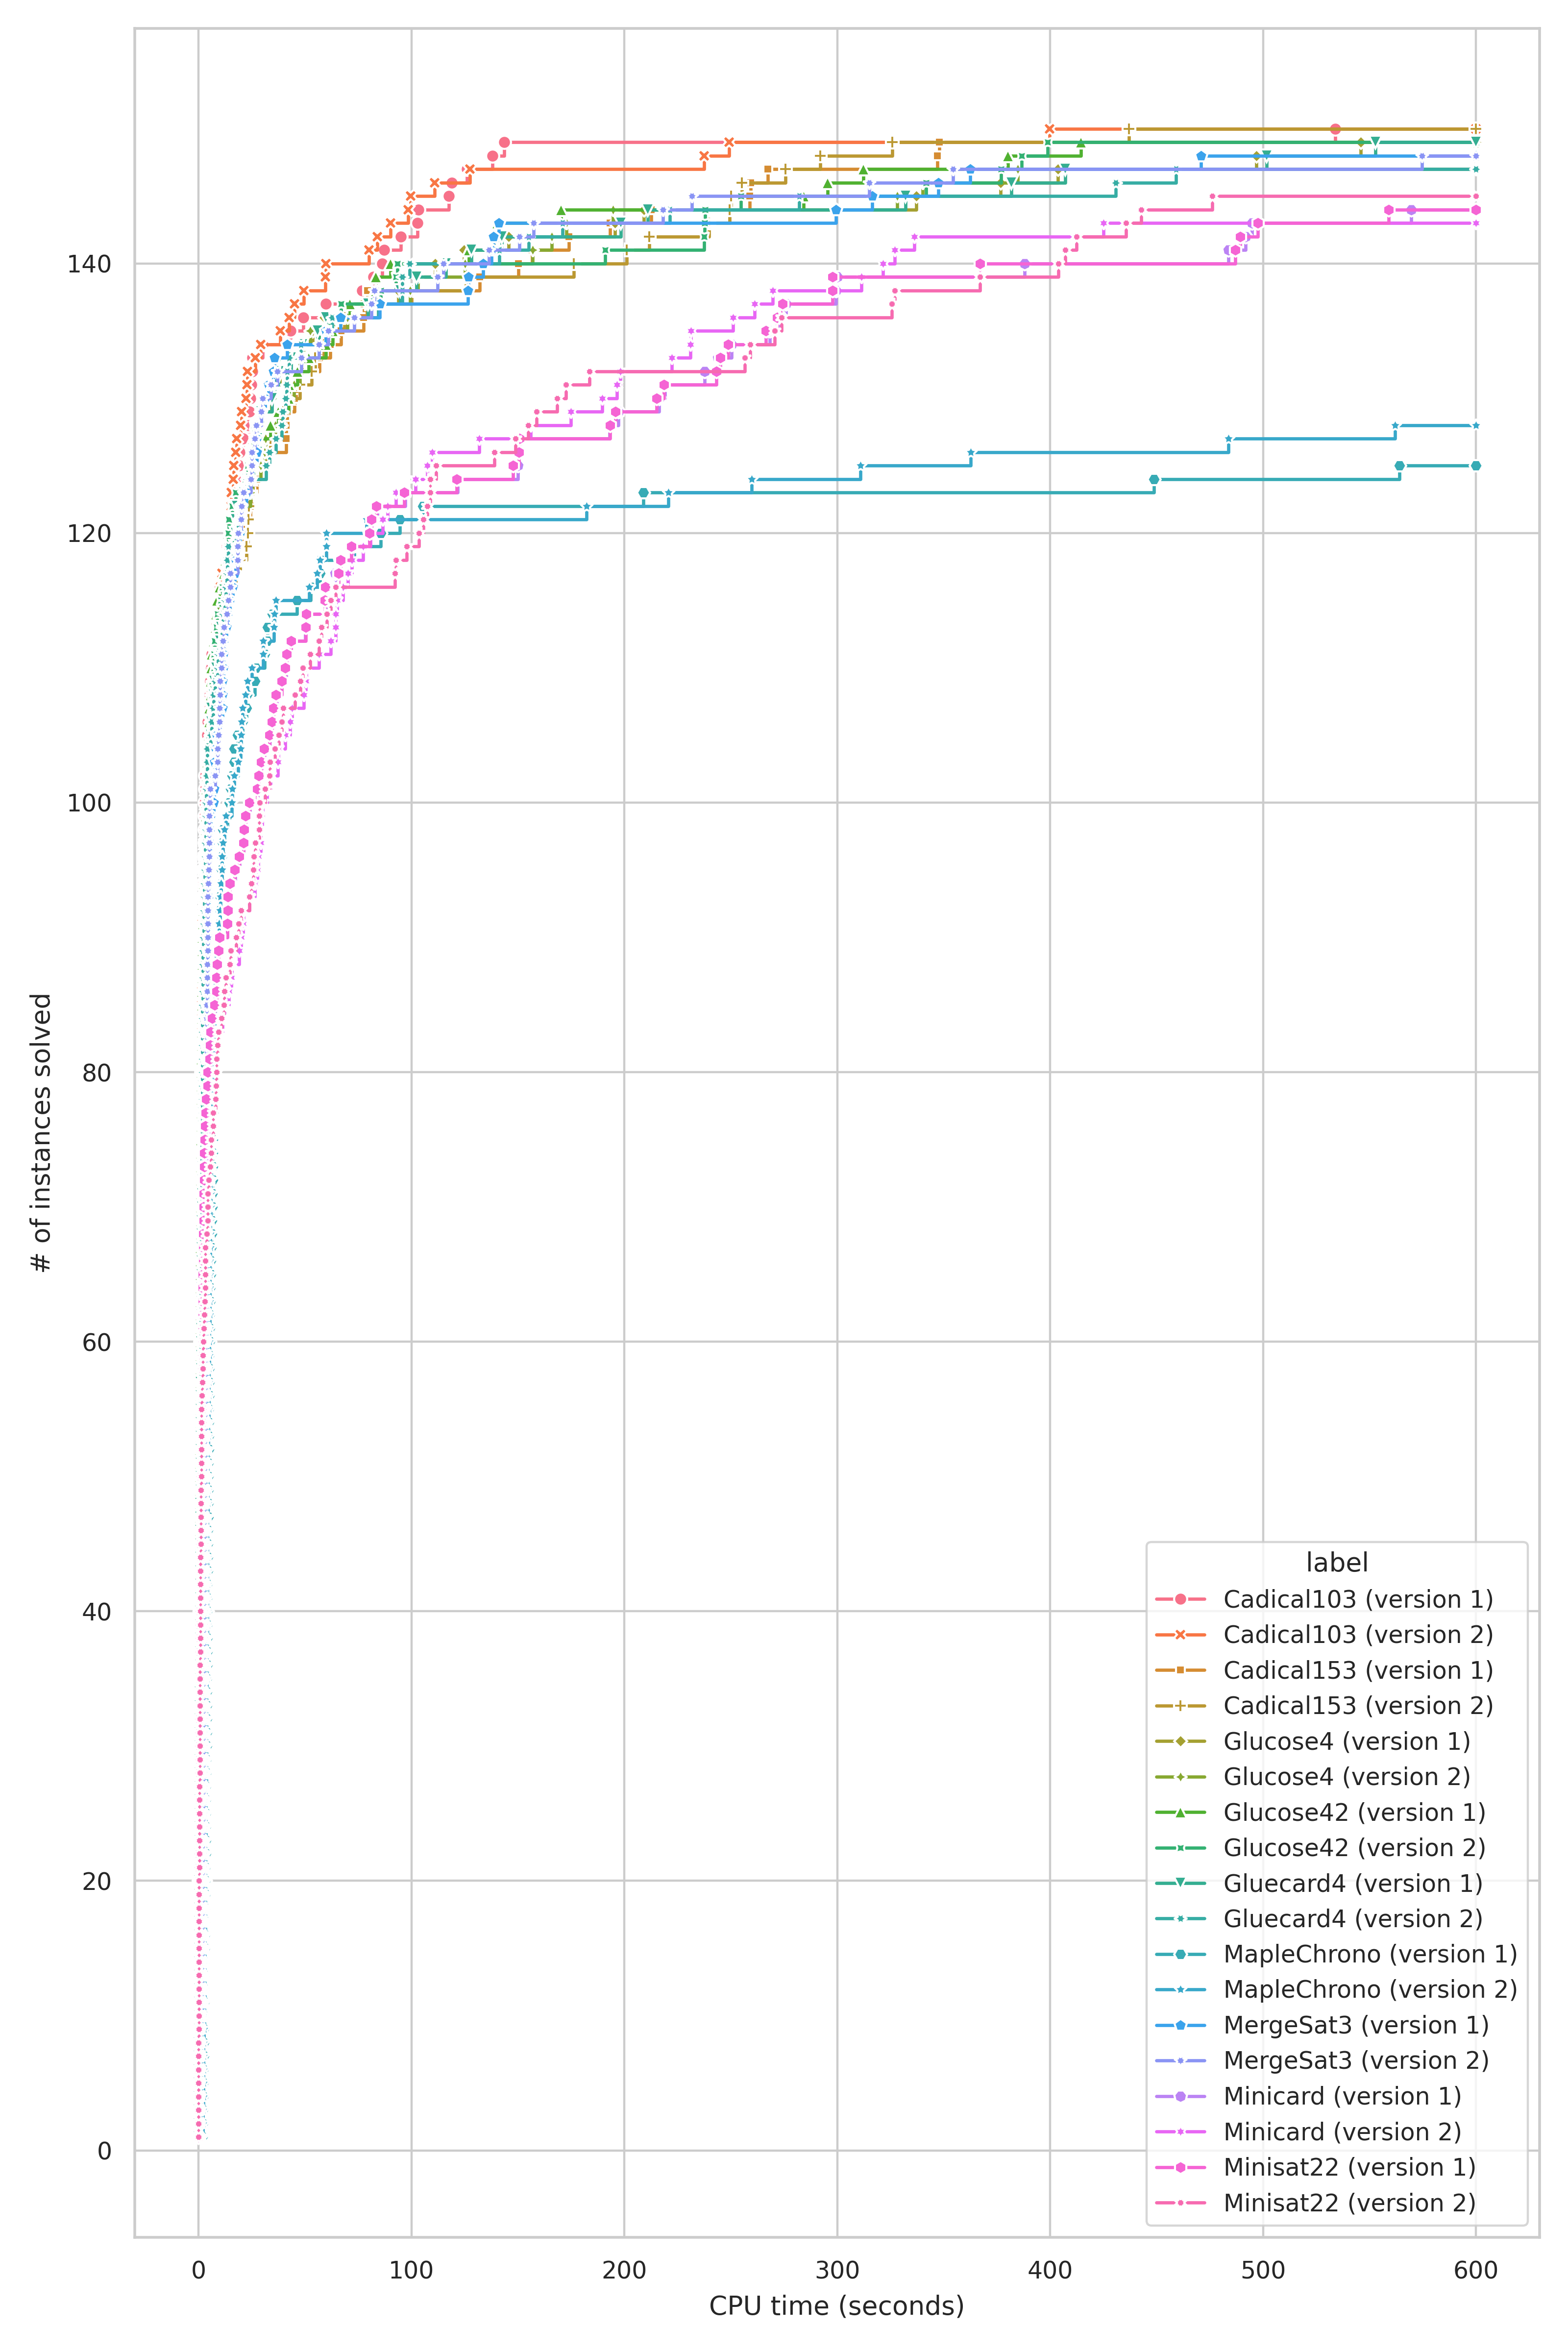
\includegraphics[scale=0.7]{Thesis/figures/minibenchmark_cactus_plot_runtime_SAT_with_holes.png}
\caption{Cactus Plot Comparing the SAT Solver Performance}
\label{fig:cactus_SAT}
\end{figure}

\begin{tabular}{llrrrrrrr}
\toprule
 &  & Cadical103 & Cadical153 & Glucose4 & Glucose42 & MergeSat3 & Minicard & Minisat22 \\
vertices & holes &  &  &  &  &  &  &  \\
\midrule
100 & 10 & 4 & 0 & 1 & 3 & 0 & 2 & 1 \\
\cline{1-9}
200 & 20 & 2 & 2 & 4 & 6 & 0 & 1 & 1 \\
\cline{1-9}
300 & 30 & 7 & 3 & 0 & 2 & 1 & 1 & 0 \\
\cline{1-9}
400 & 40 & 5 & 1 & 3 & 6 & 0 & 0 & 0 \\
\cline{1-9}
500 & 50 & 4 & 0 & 1 & 3 & 0 & 2 & 0 \\
\cline{1-9}
\bottomrule
\caption{Number instances with the lowest runtime for version1 solvers}
\end{tabular}

% \begin{tabular}{llrrrrrrrrr}\label{tab:SAT_small_time_v2}
% \toprule
%  & & Cadical103 & Cadical153 & Glucose4 & Glucose42 & Gluecard4 & MapleChrono & MergeSat3 & Minicard & Minisat22 \\
% vertices & holes &  &  &  &  &  &  &  &  &  \\
% \midrule
% 100 & 10 & 3 & 2 & 0 & 4 & 2 & 0 & 0 & 3 & 5 \\
% \cline{1-11}
% 200 & 20 & 6 & 1 & 1 & 2 & 2 & 0 & 1 & 0 & 1 \\
% \cline{1-11}
% 300 & 30 & 9 & 2 & 1 & 2 & 1 & 0 & 0 & 0 & 1 \\
% \cline{1-11}
% 400 & 40 & 3 & 3 & 1 & 3 & 4 & 0 & 0 & 1 & 0 \\
% \cline{1-11}
% 500 & 50 & 10 & 0 & 1 & 4 & 1 & 2 & 1 & 0 & 1 \\
% \cline{1-11}
% \bottomrule
% \caption{Number instances with lowest runtime for version2 solvers}
% \end{tabular}

\section{CP-SAT Formulation Comparison}
In this section, we will compare using the MIP formulation against the SAT formulation with and without the clauses \cref{eq_SAT:f.3}(CAGP)/\cref{eq_SAT_cf:f.3}(CFCAGP) for the CP-SAT solver. 

\section{MIP Parameter Set}
Gurobi allows us to set various parameters, which can help improve the runtime of the solver depending on the model. During testing, we used the model.tune() function on a few handpicked instances to determine a good parameter set. Note that setting the parameters drastically improves the runtime of the solver and one might want to further improve them in the future. In the following, we will list the parameters used for the CAGP MIP solver:
\begin{itemize}
  \item 
  \item 
  \item 
\end{itemize}
In the following, we will list the parameters used for the CFCAGP MIP solver:
\begin{itemize}
  \item 
  \item 
  \item 
\end{itemize}

\section{MIP vs. SAT vs. CP-SAT}
In this section, we will compare the performance of the MIP, SAT, and CP-SAT solver against each other on various polygon types.

\subsection{Simple Polygons}

\subsection{Orthogonal Polygons}

\subsection{Simple Polygons with Holes}

\subsection{Random von Koch Polygons}
